
\documentclass[sigconf,nonacm]{acmart}
\usepackage{graphicx}
\usepackage{rotating}
\usepackage{tikz}
\usepackage{float}
\usepackage{hyperref}
\usepackage[most]{tcolorbox}
\usepackage{cuted}
\usepackage[ruled,vlined,linesnumbered]{algorithm2e}
\usepackage{flafter}
\usetikzlibrary{positioning, arrows.meta, fit, backgrounds, calc}
\usepackage{pgfplots}
\pgfplotsset{compat=1.18}
\usepgfplotslibrary{groupplots}

% ── Architecture-diagram colours ──
\definecolor{stgI}{HTML}{9DC3E6}
\definecolor{stgII}{HTML}{5B9BD5}
\definecolor{stgIII}{HTML}{2E75B6}
\definecolor{cdraw}{HTML}{1A5276}
\definecolor{afill}{HTML}{F4B183}
\definecolor{adraw}{HTML}{C44E00}
\definecolor{ffill}{HTML}{A9D18E}
\definecolor{fdraw}{HTML}{1D7A2F}
\definecolor{hfill}{HTML}{BFBFBF}
\definecolor{hdraw}{HTML}{404040}
\definecolor{notecol}{HTML}{333333}
\definecolor{sefill}{HTML}{D5A6E6}
\definecolor{sedraw}{HTML}{7B2D8E}

\settopmatter{printacmref=false, printfolios=true}
\setcopyright{none}
\renewcommand\footnotetextcopyrightpermission[1]{}
\pagestyle{plain}
\begin{document}

\title{RepNet: Risk Estimation of Preeclampsia with Convolutional Networks and Decision Trees on 12-Lead Electrocardiograms}

\author{Ahmed Khan}
\email{aekhan@ucdavis.edu}
\affiliation{%
  \institution{UC Davis}
  \city{Davis, CA}
  \country{USA}
}

\author{Lawrencedel Legaspi}
\email{lawlegaspi@ucdavis.edu}
\affiliation{%
  \institution{UC Davis}
  \city{Davis, CA}
  \country{USA}
}

\author{Selena Phu}
\email{slphu@ucdavis.edu}
\affiliation{%
  \institution{UC Davis}
  \city{Davis, CA}
  \country{USA}
}

\begin{abstract}
  More than 76,000 women die yearly from preeclampsia and hypertensive disorders of pregnancy~\cite{butler_ai-based_2024}. We present RepNet, a pair of machine learning models for risk estimation of preeclampsia from 12-lead electrocardiogram (ECG) waveforms. One model is a depthwise-separable convolutional neural network with cross-lead multi-head self-attention and squeeze-excitation layers. In parallel we have RepNet-RF, a decision-tree ensemble with hand-engineered features extracted via NeuroKit2 and GE MUSE-reported measurements, combined with SVM and logistic regression through unweighted voting. Both models were evaluated on a dataset of 2,178 ECGs (335 PreE-positive, 15.4\% prevalence) of 1,383 unique patients from UC Davis Health using stratified group $k$-fold cross-validation. Our best CNN architecture, RepNet-SE (65,748 parameters), achieves an AUROC of 0.787. RepNet-RF reaches an AUROC of $0.757 \pm 0.039$. Gradient-based saliency maps converge on clinically relevant regions including ST-segment and T-wave, consistent with the QTc prolongation documented in PreE literature~\cite{aboshady_qtc_2025, angeli_novel_2015}.
\end{abstract}

\maketitle

{%
\renewcommand{\contentsname}{Table of Contents}
\setcounter{tocdepth}{2}
}

\section*{Code Availability}
\begin{center}
\begin{tabular}{@{}ll@{}}
\toprule
\textbf{Repository} & \textbf{Link} \\
\midrule
RepNet & \url{https://GitHub.com/AhmedKhan-GH/repnet} \\
Caliper & \url{https://GitHub.com/AhmedKhan-GH/caliper} \\
\bottomrule
\end{tabular}
\end{center}

% ══════════════════════════════════════════════════════════════
\section{Introduction}
\label{sec:intro}

Preeclampsia (PreE) is a hypertensive disorder of pregnancy that affects 2\%--8\% of pregnancies worldwide~\cite{ozcan_preeclampsia_2025}. More than 76,000 women die yearly from preeclampsia and related hypertensive disorders~\cite{butler_ai-based_2024}, and the burden falls disproportionately on developing countries where access to prenatal care is limited. PreE can progress rapidly to eclampsia, organ failure, and maternal or fetal death, yet its onset is difficult to predict from routine clinical markers alone. Current screening relies on blood pressure measurement, urine protein tests, and blood panels --- none of which reliably identify at-risk patients before symptoms appear~\cite{noauthor_preeclampsia_2018}.

The standard 12-lead electrocardiogram (ECG) is a compelling candidate for early screening. ECGs are inexpensive, non-invasive, and already routine in many clinical settings. Recent work has shown that preeclampsia induces measurable cardiac changes, including QTc prolongation and altered ventricular repolarization~\cite{raffaelli_pre-eclampsia_2014, angeli_novel_2015}. Butler et al.\ demonstrated that a modified ResNet CNN trained on raw 12-lead ECG waveforms can detect preeclampsia with an AUROC of 0.85 on a holdout set and 0.81 on an external validation cohort~\cite{butler_ai-based_2024}. Their earlier conference paper showed predictive capability up to 10 days before diagnosis~\cite{butler_electrocardiographic_2023}. These results establish that ECG signals carry discriminative information for PreE, but the approach has not been replicated on independent cohorts or with alternative architectures.

We present RepNet, a system with two complementary approaches for PreE risk estimation from 12-lead ECGs. The first is RepNet-SE, a lightweight convolutional neural network (65,748 parameters) that operates directly on raw waveforms. It uses multi-scale depthwise-separable convolutions, squeeze-and-excitation channel recalibration, and cross-lead multi-head self-attention to capture both intra-lead morphology and inter-lead dependencies. The second is RepNet-RF, a decision-tree ensemble that classifies using hand-engineered features extracted via NeuroKit2 and GE MUSE-reported measurements, combined with SVM and logistic regression through unweighted voting.

Both models were evaluated on a dataset of 2,178 ECGs (335 PreE-positive, 15.4\% prevalence) from 1,383 unique patients at UC Davis Health. We use patient-grouped stratified splitting to prevent data leakage and evaluate across multiple random seeds to measure stability. RepNet-SE achieves an AUROC of 0.787 on raw waveforms. RepNet-RF reaches an AUROC of $0.757 \pm 0.039$ on engineered features. Gradient-based saliency maps show that RepNet-SE attends to clinically relevant ECG regions including the ST-segment and T-wave, consistent with the QTc prolongation documented in PreE literature~\cite{aboshady_qtc_2025}. Our results demonstrate that raw ECG waveforms carry discriminative PreE signal and that both deep learning and classical machine learning methods can detect positive cases directly. Early screening before the onset of severe symptoms could reduce maternal and infant mortality.

% ══════════════════════════════════════════════════════════════
\section{Related Work}
\label{sec:related}

\subsection{ECG-Based Preeclampsia Detection}
% TODO: Butler et al. (2024), Adedinsewo et al. (2021)

\subsection{Deep Learning on Small ECG Datasets}
% TODO: Transfer learning paradigms, train-from-scratch tradeoffs

\subsection{Architecture Components}

\paragraph{Squeeze-and-Excitation (SE) Blocks.}
% TODO: Hu et al. (2018), IncepSE (2023)

\paragraph{Multi-Scale Convolutions.}
% TODO: InceptionTime (2020), physiological motivation

\paragraph{Depthwise-Separable Convolutions.}
% TODO: Xception (2017), MobileNet (2017), parameter reduction

\paragraph{Cross-Lead Attention.}
% TODO: MLBF-Net, GNN approaches, EfficientECG

\subsection{Regularization for Small Clinical Datasets}
% TODO: Focal loss, label smoothing, mixup, ECG augmentations


% ══════════════════════════════════════════════════════════════
\section{Dataset}
\label{sec:dataset}

\subsection{Data Source}
% TODO: Clinical 12-lead ECGs, 250 Hz, GE/Marquette, 656 vendor features

\subsection{Cohort Statistics}
% TODO: Table — total ECGs, unique patients, PE prevalence, class imbalance

\subsection{Preprocessing Pipeline}
% TODO: Baseline wander removal, powerline notch, z-score normalization
% TODO: Figure — preprocessing stages on synthetic ECG


% ══════════════════════════════════════════════════════════════
\section{Methods}
\label{sec:methods}

\subsection{RepNet-SE Architecture}
\label{sec:arch}
% TODO: Architecture overview paragraph
% TODO: Architecture diagram (TikZ)

\subsubsection{Per-Lead Weight Sharing}
% TODO: Shared conv weights across 12 leads, parameter savings, data multiplication

\subsubsection{Multi-Scale Depthwise-Separable Convolution (Stage 1)}
% TODO: Parallel DSConv branches (k=5,9,15) + maxpool branch
% TODO: Equations — branch outputs, concatenation, 1x1 projection

\subsubsection{Squeeze-and-Excitation (SE) Blocks}
% TODO: Global avg pool -> FC -> ReLU -> FC -> Sigmoid -> channel scaling
% TODO: Equation — squeeze, excitation, recalibration

\subsubsection{Cross-Lead Multi-Head Self-Attention}
% TODO: AdaptiveAvgPool tokenization, MHA across 12 lead tokens
% TODO: Equations — tokenization, attention + residual, sigmoid gating

\subsubsection{Stages 2--3: SE Per-Lead Blocks}
% TODO: Two DSConv + BN + skip + SE + MaxPool per stage
% TODO: Channel progression: 16 -> 32 -> 64

\subsubsection{Lead-Attention Pooling and Classification Head}
% TODO: Per-lead GAP, learned attention weights, weighted sum, Linear(64->2)

\subsubsection{Parameter Count}
% TODO: Table — per-component parameter breakdown, total 65,748

\subsection{Training Pipeline}

\subsubsection{Data Augmentation}
% TODO: Gaussian noise, time shift, amplitude scaling, lead dropout, cutout, baseline wander

\subsubsection{Loss Function and Class Balancing}
% TODO: Cross-entropy with class weights, focal loss exploration

\subsubsection{Optimization}
% TODO: Adam, LR, weight decay, gradient clipping, early stopping, label smoothing

\subsubsection{Bagging}
% TODO: 5-model ensemble, probability averaging

\subsection{Evaluation Protocol}

\subsubsection{Patient-Grouped Stratified Splitting}
% TODO: Patient-level grouping to prevent leakage, stratified by PE label

\subsubsection{Monte Carlo Cross-Validation}
% TODO: 20 random seeds, 80/20 splits

\subsubsection{Metrics}
% TODO: AUROC, AUPRC, Brier score, sensitivity at 80% specificity


% ══════════════════════════════════════════════════════════════
\section{Experimental Results}
\label{sec:results}

\subsection{Architecture Selection (Phase 1)}
% TODO: Table — config variants, scout seeds, mean AUROC + std

\subsection{Additional Regularization Exploration}
% TODO: Stronger regularization hurt performance

\subsection{Full Evaluation (Phase 2)}
% TODO: Table — 20-seed aggregate metrics (mean, std, median, 95% CI)

\subsection{Per-Seed Results}
% TODO: Table — all 20 seeds with AUROC, AUPRC, Brier, Sens@Sp80

\subsection{Statistical Significance}
% TODO: Table — paired t-test, Wilcoxon, Cohen's d, win count


% ══════════════════════════════════════════════════════════════
\section{Ablation Studies}
\label{sec:ablation}

\subsection{Bagging Depth}
% TODO: Table — 3-bag vs 5-bag vs 7-bag

\subsection{Early Stopping Criterion}
% TODO: AUROC-based vs AUPRC-based stopping

\subsection{Regularization Strength}
% TODO: Table — dropout / weight decay / label smoothing ablation


% ══════════════════════════════════════════════════════════════
\section{Model Analysis}
\label{sec:analysis}

\subsection{Embedding Geometry}
% TODO: PCA and t-SNE of 64-d GAP embeddings
% TODO: Figures — PCA/t-SNE colored by class and by predicted probability

\subsection{Lead Attention Weights}
% TODO: Which leads the network prioritizes

\subsection{SE Channel Importance}
% TODO: Per-channel scaling factors, PE-positive vs PE-negative

\subsection{Gradient-Based Saliency Maps}
% TODO: Input-gradient saliency, per-sample explanations
% TODO: Clinical significance — ST/T-wave regions

\subsection{Activation Propagation}
% TODO: Layer-by-layer feature maps through stages

\subsection{Cross-Lead Attention Maps}
% TODO: Attention matrices, inter-lead information flow


% ══════════════════════════════════════════════════════════════
\section{RepNet-RF}
\label{sec:rf}

\subsection{Feature Engineering}
% TODO: Neurokit ECG features — P-wave, QT, ST, axis
% TODO: Table — feature equations
% NOTE: Lawrence's work — NeuroKit2-based feature extraction pipeline

\subsection{MUSE Feature Comparison}
% TODO: Neurokit vs MUSE validation
% TODO: Tables — feature performance comparison

\subsection{Ensemble Voting Results}
% TODO: RF + SVM + LR unweighted voting performance
% TODO: Chi-squared feature importance
% NOTE: RepNet-RF — RF, SVM, LR with unweighted voting


% ══════════════════════════════════════════════════════════════
\section{Discussion}
\label{sec:discussion}

\subsection{RepNet-SE vs.\ RepNet-RF}
% TODO: Central finding — AUROC comparison, stability across configs

\paragraph{Dataset Size.}
% TODO: 2,178 ECGs vs. 656 features as implicit dimensionality reduction

\paragraph{Signal-to-Noise Ratio.}
% TODO: Subtle PE changes, vendor algorithms vs learned feature extraction

\paragraph{Inductive Bias vs. Data.}
% TODO: Architectural priors cannot compensate for limited data

\subsection{Comparison with Literature}
% TODO: Butler et al. context — different cohort, protocol, severity

\subsection{Parameter Efficiency}
% TODO: 65K vs 280K (ResNet) vs 965K (CrossLead Deeper)

\subsection{Clinical Implications}
% TODO: Best seeds show signal exists
% TODO: RepNet-RF as practical clinical tool, neural approach for raw-signal settings

\subsection{Limitations}
% TODO: Single-site, no pretraining, fixed length, no demographics, cross-sectional


% ══════════════════════════════════════════════════════════════
\section{Conclusion}
\label{sec:conclusion}

% TODO: Summary — architecture, results, comparison
% TODO: Future work — larger datasets, transfer learning, ECG foundation models
% TODO: Caliper demonstration at Senior Design Showcase


% ══════════════════════════════════════════════════════════════
\bibliographystyle{ACM-Reference-Format}
\bibliography{project_references}

\appendix

\section{RepNet-SE Architecture Diagram}
\label{sec:arch-diagram}

\begin{figure*}[h]
  \centering
  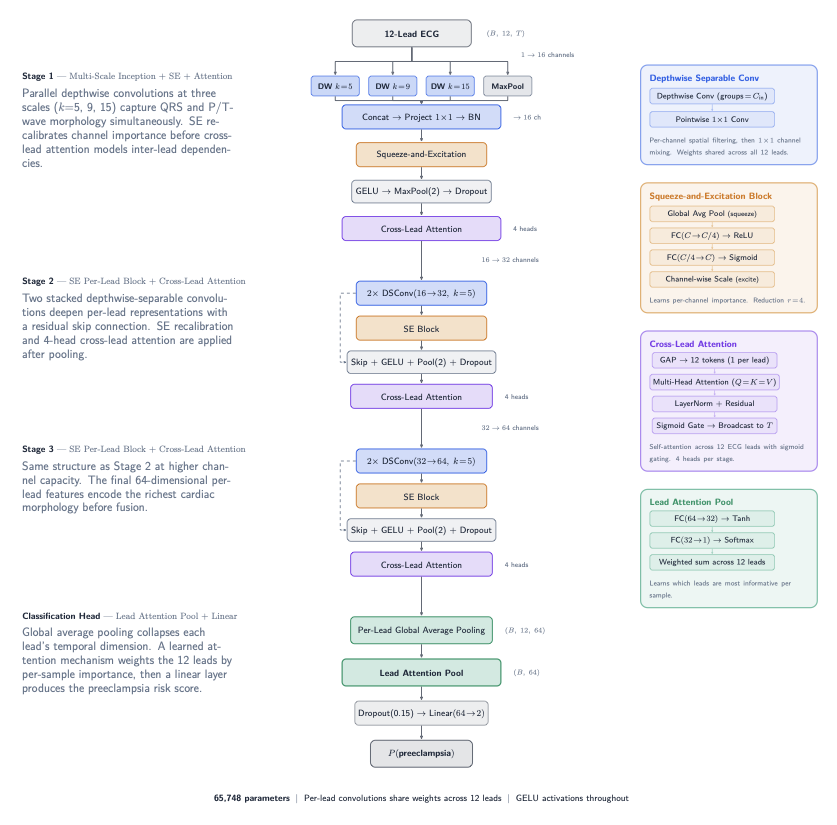
\includegraphics[width=\textwidth]{architecture/repnet_se_architecture.pdf}
  \caption{RepNet-SE architecture: multi-scale depthwise-separable convolutions
    with squeeze-and-excitation and cross-lead attention across three stages,
    followed by a lead attention pool and linear classifier (65,748 parameters).}
  \label{fig:arch-diagram}
\end{figure*}

\end{document}
